\chapter{Finite Elements in Time}\label{cha:finite elements in time}
    \BA{Introduction.}

    Traditional approaches for discretizing time-dependent PDEs, $\partial_{t}u  =  \calF(u)$, through the FE method cast the PDE into a weak form by testing against test functions, $v$, on the $d$-dimensional, polygonal, spatial domain $\bfOmega$, as ``$\langle\partial_{t}u, v\rangle$''  $=  \langle\calF(u), v\rangle$, where the choice of interpretation of the time derivative term ``$\langle\partial_{t}u, v\rangle$'', typically through a generic Runge–Kutta (RK) method, characterises the timestepper for the scheme. For traditional FE software designed for solving FE problems in space only, these techniques can be implemented through manually-implemented loops on each timestep, or through specialist packages when available, such as the \texttt{Irksome} package within \texttt{Firedrake} \BA{[Ref]}.

    An alternative approach—FEs in time—interprets the PDE on the domain $\bfOmega\otimes T$, where $T$ represents a time interval, potentially the timestep $\left[t^{k}, t^{k + 1}\right]$ or the whole interval to be considered. One then tests against test functions, $v$, defined equally over the whole domain $\bfOmega\otimes T$, as $\langle\partial_{t}u, v\rangle  =  \langle\calF(u), v\rangle$. The original ambiguity in interpretation of the time derivative term, ``$\langle\partial_{t}u, v\rangle$'', when picking the RK scheme is transferred to the choice of behavior, continuity, order etc. of the finite element discretizations in the time domain. A few key points on this formulation:
    \begin{itemize}
        \item  Such FE spaces can be constructed via the tensor product of FE spaces on $d$-dimensional $\bfOmega$ and 1-dimensional $T$, without needing to construct FE spaces on the entire $(d + 1)$-dimensional domain $\bfOmega\otimes T$.
        \item  Akin to Petrov–Galerkin methods, the test function space need not be identical to the trial function space, and often won't be:- for PDEs that are 1$^{\text{st}}$-order in time, for example, a typical weak formulation will require high regularity in the trial space than the test space (see $\langle\partial_{t}u, v\rangle$) which will then typically be reflected in the choice of FE discretizations.
        \item  When using a FE-in-time interpretation, the intention is typically \emph{not} to solve a highly computationally intense, $(n + 1)$-dimensional FE problem on all of $\bfOmega\otimes T$, but to extract a timestepper from the distretization that need only be solved on the $d$-dimensional spatial domain, $\bfOmega$, by exploiting block-triangularity in the stiffness \BA{(Is this the right terminology here?)} matrix. It is in fact often the case that the resultant timesteppers are identical to those that would be derived from a RK-scheme interpretation.
    \end{itemize}

    \BA{Should list some pros/cons from my reading group FET presentation.}

    \BA{I say ``typically'' a \emph{lot} here...}

    \line
    
    \begin{example}
        Consider the heat equation on $\bfOmega\otimes T$,
        \begin{equation}\label{eqn:FEs in time PDE}
            \partial_{t}u  =  \kappa\Delta u,
        \end{equation}
        with boundary conditions on $\bfGamma  :=  \bfOmega$,
        \begin{equation}\label{eqn:FEs in time BC}
            u  =  0|_{\bfx \in \bfGamma},
        \end{equation}
        and initial conditions at $t  =  0$,
        \begin{equation}\label{eqn:FEs in time IC}
            u  =  u_{0}|_{t = 0}.
        \end{equation}
        
        Testing against $v$ supported on $\bfOmega\otimes T$ casts (\ref{eqn:FEs in time PDE}) into a chosen weak formulation:
        \begin{align}
            \langle\partial_{t}u, v\rangle_{\bfOmega\otimes T}  &=  \kappa\langle\Delta u, v\rangle_{\bfOmega\otimes T}  \\
                                                                &=   - \kappa\langle\nabla u, \nabla v\rangle_{\bfOmega\otimes T}  \impliedby  {\rm (\ref{eqn:FEs in time BC})}
        \end{align}
        To solve this via FEs in time therefore, we seek $u^{h}  \in  \bbU^{h}$ such that $\forall  v^{h}  \in  \bbV^{h}$,
        \begin{equation}\label{eqn:FEs in time weak form}
            \left\langle\partial_{t}u^{h}, v^{h}\right\rangle_{\bfOmega^{h}\otimes T^{h}}  =  - \kappa\left\langle\nabla u^{h}, \nabla v^{h}\right\rangle_{\bfOmega^{h}\otimes T^{h}}
        \end{equation}
        Let $\bfOmega^{h}$ be a mesh of simplicies on $\bfOmega$, and $T^{h}$ be a mesh of equal intervals on $T$. Using an order-$p$ ``CG'' method (in space), with an order-$q$ timestepper, define:
        \begin{align}
            \bbU^{h}  :=  \bbP_{p}\left(\bfOmega^{h}\right)\otimes\bbP_{q}\left(T^{h}\right),  &&
            \bbV^{h}  :=  \bbP_{p}\left(\bfOmega^{h}\right)\otimes\bbDP_{q - 1}\left(T^{h}\right)
        \end{align}
        Denote bases for these FE spaces:
        \begin{align}
            (\psi_{i})_{i}     \text{ for }  \bbP_{p}\left(\bfOmega^{h}\right),  &&
            (\phi_{i})_{i}     \text{ for }  \bbP_{q}\left(T^{h}\right),         &&
            (\varphi_{i})_{i}  \text{ for }  \bbDP_{q - 1}\left(T^{h}\right)
        \end{align}
        $u^{h}$, $v^{h}$ can be expressed in terms of these bases as:
        \begin{align}
            u^{h}(\bfx; t)  =  \sum_{k, l}u_{kl}\psi_{k}(\bfx)\phi_{l}(t),  &&
            v^{h}(\bfx; t)  =  \sum_{i, j}v_{ij}\psi_{i}(\bfx)\varphi_{j}(t)
        \end{align}
        Substituting into (\ref{eqn:FEs in time weak form}), $\forall  v_{kl}$:
        \begin{multline}
            \left\langle\partial_{t}\left[\sum_{k, l}u_{kl}\psi_{k}(\bfx)\phi_{l}(t)\right], \sum_{i, j}v_{ij}\psi_{i}(\bfx)\varphi_{j}(t)\right\rangle_{\bfOmega^{h}\otimes T^{h}}  \\
            =  - \kappa\left\langle\nabla\left[\sum_{k, l}u_{kl}\psi_{k}(\bfx)\phi_{l}(t)\right], \nabla\left[\sum_{i, j}v_{ij}\psi_{i}(\bfx)\varphi_{j}(t)\right]\right\rangle_{\bfOmega^{h}\otimes T^{h}}
        \end{multline}
        \begin{equation}
            \sum_{i, j, k, l}v_{ij}\langle\psi_{i}, \psi_{k}\rangle_{\bfOmega^{h}}\langle\varphi_{j}, \partial_{t}\phi_{l}\rangle_{T^{h}}u_{kl}  =  - \kappa\sum_{i, j, k, l}v_{ij}\langle\nabla\psi_{i}, \nabla\psi_{k}\rangle_{\bfOmega^{h}}\langle\varphi_{j}, \phi_{l}\rangle_{T^{h}}u_{kl}
        \end{equation}
        Denoting the vectors $\bfu  :=  (u_{kl})_{kl}$, $\bfv  :=  (v_{ij})_{ij}$, this takes the matrix form
        \begin{equation}
            \bfv^{T}(\langle\psi_{i}, \psi_{k}\rangle_{\bfOmega^{h}}\langle\varphi_{j}, \partial_{t}\phi_{l}\rangle_{T^{h}})_{i, j}^{k, l}\bfu  =  \kappa\bfv^{T}(\langle\nabla\psi_{i}, \nabla\psi_{k}\rangle_{\bfOmega^{h}}\langle\varphi_{j}, \phi_{l}\rangle_{T^{h}})_{i, j}^{k, l}\bfu.
        \end{equation}
        Indexing vectors first in the time indices $j$ and $l$, this simplifies to
        \begin{equation}
            \bfv^{T}\left[(\langle\varphi_{j}, \partial_{t}\phi_{l}\rangle_{T^{h}})_{j}^{l}\otimes\bfM + \kappa(\langle\varphi_{j}, \phi_{l}\rangle_{T^{h}})_{j}^{l}\otimes\bfK\right]\bfu  =  0
        \end{equation}
        where $\bfM$ and $\bfK$ respectively denote the mass and stiffness matrices:
        \begin{align}
            \bfM  :=  (\langle\psi_{i}, \psi_{k}\rangle_{\bfOmega^{h}})_{i}^{k},  &&
            \bfK  :=  (\langle\nabla\psi_{i}, \nabla\psi_{k}\rangle_{\bfOmega^{h}})_{i}^{k},
        \end{align}
        and $\otimes$ denotes the matrix Kronecker product.
        
        Regarding the sparsity of this matrix, with appropriate ordering of the bases $(\phi_{i})_{i}$, $(\varphi_{i})_{i}$, the matrices $(\langle\varphi_{j}, \partial_{t}\phi_{l}\rangle_{T^{h}})_{j}^{l}$, $(\langle\varphi_{j}, \phi_{l}\rangle_{T^{h}})_{j}^{l}$ take the general form
        \begin{equation}\label{eqn:timestepper matrices}
            \left(\begin{array}{ c : c c : c c : c c }
                \pm\bfb  &  \bfA    &  \bfb     &  0       &  0        &  \cdots   &  0        \\
                \hdashline
                0        &  0       &  \pm\bfb  &  \bfA    &  \bfb     &  \cdots   &  0        \\
                \hdashline
                0        &  0       &  0        &  0       &  \pm\bfb  &  \cdots   &  0        \\
                \hdashline
                \vdots   &  \vdots  &  \vdots   &  \vdots  &  \vdots   &  \ddots   &  \vdots   \\
                \hdashline
                0        &  0       &  0        &  0       &  0        &  \cdots   &  \bfb     \\
            \end{array}\right)
        \end{equation}
        for some $\bfA  \in  \bbR^{q\times (q - 1)}$, $\bfb  \in  \bbR^{q}$ in either case, dependent on the choice of bases. (See Figure \ref{fig:timestepper matrices}) \BA{(Capitalization on ``Figure''?)}

        \begin{figure}[!ht]
            \centering
            \begin{subfigure}{0.5\textwidth}
                \centering
                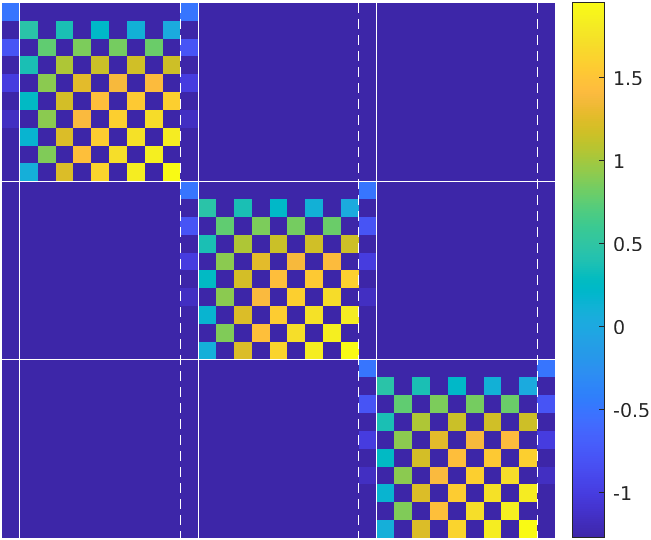
\includegraphics[width = 0.9\textwidth]{9 - finite elements in time/images/matrix 1.png}
                \caption{$(\langle\varphi_{j}, \partial_{t}\phi_{l}\rangle_{T^{h}})_{j}^{l}$}
            \end{subfigure}%
            \begin{subfigure}{0.5\textwidth}
                \centering
                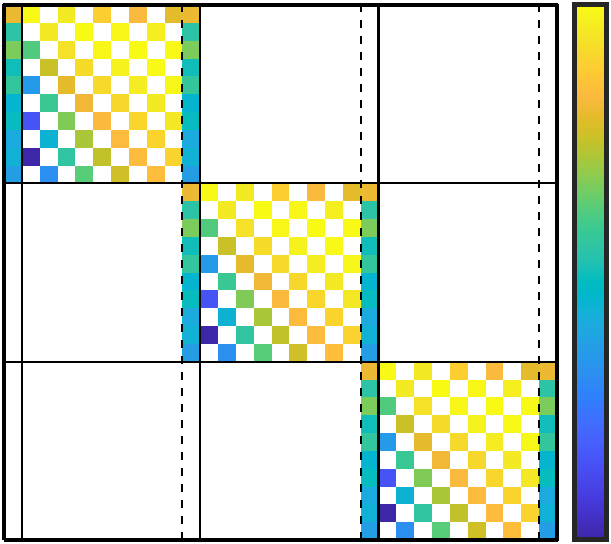
\includegraphics[width = 0.9\textwidth]{9 - finite elements in time/images/matrix 2.png}
                \caption{$(\langle\varphi_{j}, \phi_{l}\rangle_{T^{h}})_{j}^{l}$}
            \end{subfigure}
            \caption{Sparsity plots for the two timestepping matrices when $q = 10$ on 3 (equal) intervals, under simple normalised polynomial bases. \\ Color indicates $\log(|*|)$ for the matrix entries. Black lines indicate block structure from (\ref{eqn:timestepper matrices}), while solid black lines highlight the lower-block-triangular structure after elimination of first column.}
            \label{fig:timestepper matrices}
        \end{figure}

        With strongly-imposed initial conditions on $\bbU^{h}$, the first column of this matrix is eliminated, leaving a lower-block-triangular matrix of size-$p$ blocks, as indicated by the dashed lines in (\ref{eqn:timestepper matrices}). Applying block forward substitution to solve this block triangular problem is perfectly analogous to using a traditional timestepper.

        Denoting, $\bfu_{l}  :=  (u_{kl})_{k}$, on the $n$-th timestep, the resultant linear problem takes the form:
        \begin{equation}
            \left[(\langle\varphi_{nq + j}, \partial_{t}\phi_{nq + l}\rangle_{T^{h}})_{j = 1, \cdots, q}^{l = 0, \cdots, q}\otimes\bfM + \kappa(\langle\varphi_{nq + j}, \phi_{nq + l}\rangle_{T^{h}})_{j = 1, \cdots, q}^{l = 0, \cdots, q}\otimes\bfK\right](\bfu_{nq + l})_{l = 0, \cdots, q}  =  \bfzero
        \end{equation}
        \begin{multline}
            \left[(\langle\varphi_{nq + j}, \partial_{t}\phi_{nq + l}\rangle_{T^{h}})_{j = 1, \cdots, q}^{l = 1, \cdots, q}\otimes\bfM + \kappa(\langle\varphi_{nq + j}, \phi_{nq + l}\rangle_{T^{h}})_{j = 1, \cdots, q}^{l = 1, \cdots, q}\otimes\bfK\right](\bfu_{nq + l})_{l = 1, \cdots, q}  \\
            =  - [(\langle\varphi_{nq + j}, \partial_{t}\phi_{nq}\rangle_{T^{h}})_{j = 1, \cdots, q}\otimes\bfM + \kappa(\langle\varphi_{nq + j}, \phi_{nq}\rangle_{T^{h}})_{j = 1, \cdots, q}\otimes\bfK]\bfu_{nq}
        \end{multline}
        which can be solved iteratively for each $\bfu_{(n + 1)q}$ at each new timestep.

        In the case of $q = 1$—the lowest-order method—with time intervals of length $\delta t$, this takes the form
        \begin{equation}
            \left[\bfM + \kappa\frac{\delta t}{2}\bfK\right]\bfu_{n + 1}  =  \left[\bfM - \kappa\frac{\delta t}{2}\bfK\right]\bfu_{n},
        \end{equation}
        which, by rearranging, can be seen to be equivalent to the traditional implicit midpoint method,
        \begin{equation}
            \bfM\left[\frac{1}{\delta t}(\bfu_{n + 1} - \bfu_{n})\right]  =  - \kappa\bfK\left[\frac{1}{2}(\bfu_{n + 1} + \bfu_{n})\right],
        \end{equation}
        or, in weak formulation,
        \begin{equation}
            \left\langle v^{h}_{n + 1}, \frac{1}{\delta t}\left(u^{h}_{n + 1} - u^{h}_{n}\right)\right\rangle_{\bfOmega^{h}}  =  - \left\langle\nabla v^{h}_{n + 1}, \frac{1}{2}\nabla\left(u^{h}_{n + 1} + u^{h}_{n}\right)\right\rangle_{\bfOmega^{h}}.
        \end{equation}

        \BA{Would be nice to restructure this example to generally talk more in the weak formulations than with all these mass/stiffness matrices that aren't necessarily relevant to understanding how FEs in time give rise to timesteppers.}
    \end{example}

    \line

    \BA{Note about FDM bases?}
    
    \BA{Should go through and add correct punctuation to my equations.}
